\section{Áramkör terv}

A rendszer elkészítéséhez szükséges volt egy áramkör tervezése is, mivel több komponens
csak SMD (Surface Mount Component) formában találhatóak meg, így nem alkalmazhatóak egy
egyszerű breadboard. Ezen megtalálható minden ami szükséges a rendszer működéséhez, 
csupán egy micro-USB szükséges a rendszer táplálásához.

Az áramkör tervet az EasyEDA-ban terveztem, ez egy ingyenesen használható szerkesztő
program, akár webes felületen is használható és nagy mennyiségű alkatrész található
meg az adatbázisában amelyek a tervezésre használhatóak.

Az áramkör egy kétoldalas lapon található és csak egy oldalán találhatóak a komponensek.
A másik oldalán legfőképpen a huzalozás található. A rendszer használ kis méretű
SMD alkatrészeket és THC alkatrészeket is. 

A huzalozás során nagyobb figyelmet fektettem a nagy frekvenciás SPI jelek
és a mérőáramkör szétválasztására, a zajok csökkentése érdekében.

\subsection{Problémák az áramkör tervezésekor}

Mivel számomra az áramkör tervezés tárgy nem volt elérhető, így ez volt az első 
áramkör amit terveztem. Így többször át kellett alakítsam, hogy kivitelezhető legyen.

Legelső alkalommal a rendszer nem volt kivitelezhető, mivel túl vékony vezetékeket
használtam, ami nem volt legyártható a számomra elérhető helyeken. A komponenseket 
nehezen lehetett volna beilleszteni (Through Hole komponensek esetén, mint a kijelző),
mivel a vezetékek a lap mindkét oldalán voltak vezetve, így forrasztás során nehéz
lett volna azokat a lábakat forrasztani, amelyek a képernyő oldalán voltak.
Ezek át kellett vezessem olyan módon, hogy csakis a lap másik oldalán legyen a vezeték
csatlakoztatva a komponenshez.

Beszerzés során nem rendeltem meg minden alkatrészt, csak a fontosakat, így néhány
egyszerű alkatrészt helyettesítettem más alaktrésekkel, ez csupán egy feszültség referenciát
2 LED-et és egy kapcsolót érintett, így ezeket inkább helyileg helyettesítettem, minthogy
ismét rendeljem meg azokat.

A kijelző mérete a szerkesztőben és a valóságban nem egyezett meg, viszont ez még 
kiderült az áramkör kinyomtatása előtt, így nem vesztődött el sok idő. Az egész
kijelző nagyobb volt, mint a valóságban, még a láb közei is, így könnyedén látható
volt, hogy a tervrajz nem lesz kivitelezhető.

A tervrajzra nem tüntettem fel néhány jelzést, ami a felhasználást segíti, így ezt 
utólag felrajzoltam a lapra.

\subsection{Áramkör elkészítése}

Miután a tervezés elkészült és kivitelezhetőnek lett minősítve azután az áramkör
el lett keszítve az egyetemi laboratórium segítségével. Miután a lapot a furatokkal és a réz
huzalozással megkaptam azután elkezdtem a komponensek felhelyezését.

Áramkör forrasztásával szintén nem volt sok tapasztalatom, csupán egyszerűbb
áramkörökkel, így nem a lehető legszebb, viszont használat során minden elektonikailag
csatlakoztatva van, így az áramkör működőképes. A végső áramkör a következőkben néz ki.
[\ref{fig:Aramkor}]


\begin{figure}[h]
    \centering
    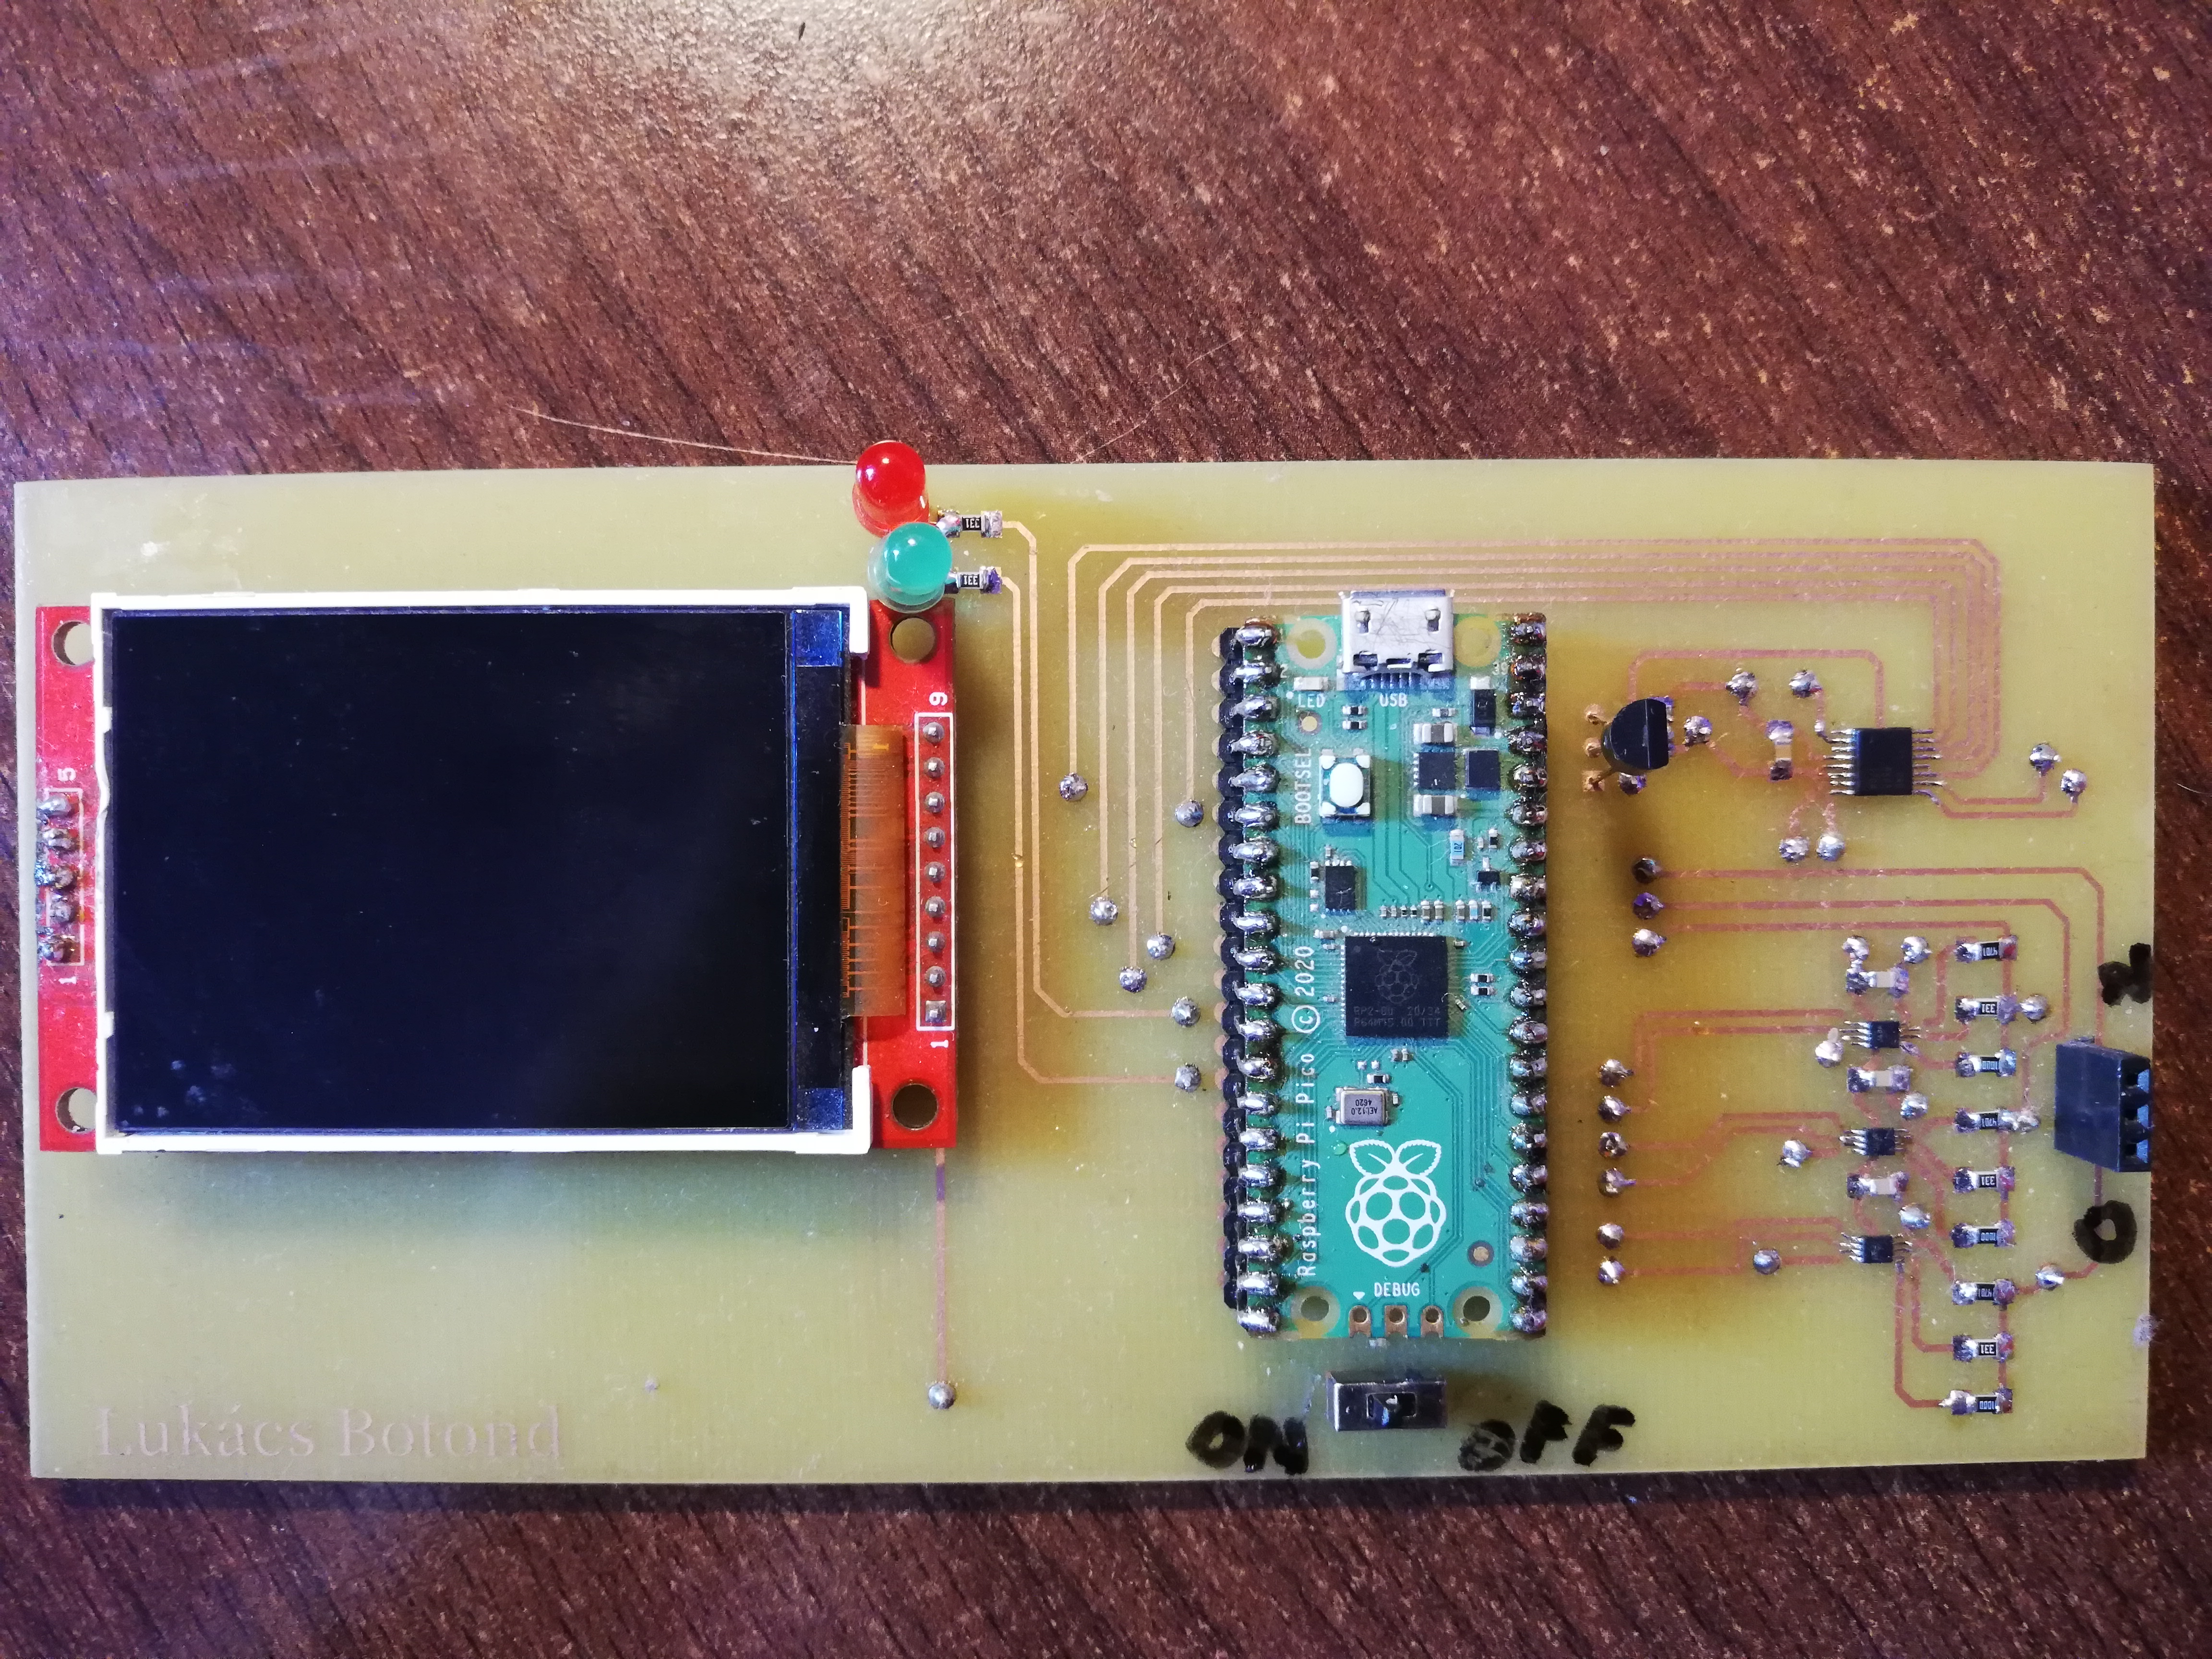
\includegraphics[scale=0.1]{images/literature/PCB.jpg}
    \caption{A kész áramkör}
    \label{fig:Aramkor}
\end{figure}

\section{Szimulációk}

A szimulációra az LTspice \cite{LTspice} alkalmazást használtam, 
amelyben felépítettem a mérő áramkört és ellenőriztem, hogy az elméleti
mérési módszer alkalmas-e a mérés elvégzésére, és az értékek milyen
tartományban vannak, mivel a rendszer nem eléggé érzékeny, hogy a precíz
értékeket pontosan megadja, így olyan módszer kell ahol a tolerancia nagyobb.
Egy ilyen példa az áramerősség mérése amit a port ellenállást használja az
áramerősség meghatározására, viszont kis ellenállás esetén a
feszültség esés az ellenálláson alacsony áram esetén nem mérhető pontosan.
Ezért ilyen esetben nagyobb port ellenállást kell alkalmazni, hogy mérhető 
legyen a feszültség esés.

A program képes az időben változó feszültségeket is mérni, így
meg lehet tudni, hogy milyen idő intervalumban kell nézni és hogy
a komponensek időben mennyire befolyásolják a mérést. Ez 
legfőképpen a kondenzátorok mérésekor volt fontos, hogy megbizonyodjak
a mérések valóságosságáról.

